
\chapter{Mes réalisations}

\section{Présentation du framework Play!}

Play! est un jeune framework qui permet de créer facilement des
applications web avec Java et Scala.
Mon stage a deux buts majeurs pour l'entreprise :

\begin{enumerate}
\item Rendre accessible à tous l'utilisation de l'outil d'infra en proposant
  une interface web ergonomique.
\item Explorer le potentiel du framework Play! pour qu'il remplace
  éventuellement du code php existant dans différents logiciels de
  l'entreprise.
\end{enumerate}

Durant mes deux premières semaines de stage, j'ai préparé des slides pour une
présentation du framework. Cette présentation met en avant les caractéristiques
de Play!, ses points forts et faiblesses, et comment il se place face aux
alternatives existantes.
L'équipe croit au potentiel du framework mais attend le résultat de
l'interface web de l'outil d'infra pour décider de remplacer le code php
existant.

La semaine suivante consiste à tester l'outil d'infra en ligne de
commande et à réfléchir à l'interface utilisateur pour l'application web (url
disponibles, dispositions des boutons et des champs de saisies).

Une nouvelle branche est ajoutée dans Mercurial pour accueillir l'application web.
Le développement peut commencer!


\section{Le déploiement}

Le déploiement doit être fonctionnel avant de développer l'application.

En effet, il se peut que les contraintes d'infrastructure empêche
le déploiement d'une application : l'espace disque dur qui peut être insuffisant
pour accueillir l'application, l'impossibilité d'ouvrir des ports http.
Nous devons donc vérifier que le déploiement fonctionne bien de bout en bout.

Pour cela, une application simpliste est créée.
Elle affiche juste une page web avec du contenu statique.

Il faut maintenant héberger l'application puis automatiser le déploiement en
programmant des scripts.

\subsection{Amazon héberge l'application}

Sur Amazon Web Services, une instance EC2 portant le nom 'infra-admin-web' est
créée. C'est en fait le serveur qui hébergera l'application. Le
système d'exploitation de cette instance est Ubuntu 12.04 .
C'est une instance de type \textit{t1.micro} qui est idéale pour le type
d'application web attendue.
En effet, les clients de l'application web seront les membres de la société.
Du fait du nombre limité d'utilisateurs, environ 25 développeurs,
une puissance CPU limitée suffit.

Une instance Micro (\textit{t1.micro}) fournit une petite quantité de ressources CPU
constantes et augmente dynamiquement sa capacité CPU sur de courtes durées
lorsque des cycles supplémentaires sont disponibles. Donc elle convient bien
aux applications à moindre trafic ou aux sites consommant un nombre de cycles
significatif périodiquement.

Le schéma suivant illustre l'utilisation CPU typique d'une application web
tournant sur une instance de type \textit{t1.micro} :
\begin{figure}[H]
  \begin{center}
    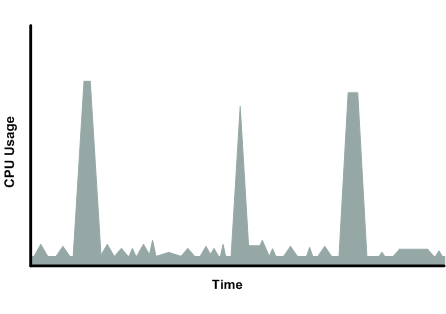
\includegraphics[scale=0.8]{cpu-usage.png} 
  \end{center}
  \caption{utilisation CPU pour une instance de type micro}
\end{figure}

Les instances de type micro sont aussi les moins chers de tous les types
d'instances proposés par Amazon. Leurs prix est de seulement 2 centimes de
dollars par heure.

\subsection{Scripts Bash}

Maintenant que nous disposons d'une instance EC2 réservée pour l'application
web, il faut automatiser les actions récurrentes qui devront être effectuées.

Quatre scripts Bash sont créés pour exécuter les taches récurrentes :
deploy.sh, start.sh, stop.sh et restart.sh pour respectivement déployer
l'application web, la démarrer, l'arrêter et la redémarrer.

deploy.sh est un script qui se trouve sur la machine local.
Ce script package l'application puis la copie sur l'instance EC2 via scp.
Les scripts start.sh, stop.sh et restart.sh se trouvent sur l'instance EC2 et
peuvent être appelés à distance via ssh.


\section{Premier concept de webapp : appeler l'outil d'infra comme une commande
  shell}
\noindent Les objectifs de la première version de la webapp sont les suivants :
\begin{enumerate}
\item La webapp exécutera l'outil d'infra en ligne de commande comme un
  programme externe.
\item La webapp doit permettre d'exécuter deux commandes en parallèle.
\end{enumerate}

Le code coté serveur est écrit en Scala.
Puisque toute classe Java peut être naturellement instanciée dans du code Scala,
c'est la classe Java ProcessBuilder qui est utilisée pour exécuter
l'outil d'infra comme programme externe.
Qu'en au code coté client, il doit afficher la sortie de la commande dans le
navigateur.

Une contrainte apparaît :
Certaines commandes de l'outil d'infra prennent beaucoup de temps à s'exécuter.
L'output de la commande doit donc être affichée au fur et à mesure de son
exécution. Pour ce faire :\\
\textit{Coté serveur}, un BufferedReader récupère dynamiquement la sortie de la commande.\\
\textit{Coté client}, du JavaScript affiche progressivement le résultat.

Le point restant est la communication entre le serveur et le navigateur du
client pour afficher dynamiquement du contenu dans la page web.

\subsection{Communications asynchrones pour une application web temps réel}

Dans une application Web traditionnelle, lorsque l'utilisateur effectue une
action, celle-ci est exécutée et le navigateur attend le résultat pour rendre
la main à l'utilisateur. Lorsque cette action requiert un calcul coûteux
au serveur, cela occasionne des délais et une attente pour le client.

Le mode asynchrone élimine cette attente. Les requêtes au serveur sont lancées
sans que soit suspendue l'interaction avec le navigateur et la page est mise à
jour lorsque les données requises sont disponibles.

La première solution bien connue pour disposer de ce comportement asynchrone est
\textit{Ajax}.
\textit{Ajax} est une technologie permettant de créer des applications qui simulent un
comportement temps réel. Le navigateur envoi une requête HTTP à intervalle
régulier et reçoit une réponse.
Il existe aujourd'hui des alternavives à \textit{Ajax} pour voir des données se mettre à
jour dans sa page web sans appuyer sur le bouton refresh.

La webapp de l'outil d'infra utilise des \textit{WebSocket}.
C'est une autre technologie web, bien plus récente, qui permet de créer de vrais
applications temps réel.
Alors que le protocole HTTP opère par une succession de requêtes et réponses
alternatives, \textit{WebSocket} est bidirectionnel : une connexion statique s'établit
entre le serveur et le client et les deux parties envoient des données à leur
convenance.
C'est un authentique canal de communication bidirectionnel (push depuis le
serveur) transparent pour les firewalls, proxy, et routeurs.
Il n'y a aucune latence réseau lors des transmission, les performances réseaux
qu'elle offre est l'un de ses gros points forts.
Le framework Play! fournit une bibliothèque complète pour utiliser les
\textit{WebSockets}.
La webapp fait donc usage des \textit{WebSockets} pour récupérer dynamiquement le
résultat de la commande et l'afficher dans le navigateur.

Pour chaque nouvelle page ouverte, une WebSocket est créée.
Deux utilisateurs peuvent alors exécuter leur commande en parallèle sans
bloquage ni intercalage des logs des commandes.

Voici une capture d'écran de l'interface web disponible avec la première version
de la webapp :
\begin{figure}[H]
  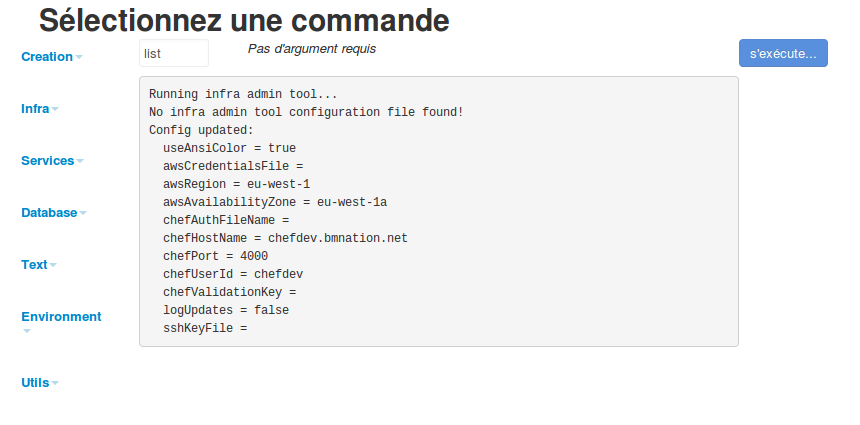
\includegraphics[width=\textwidth]{webapp-processbuilder.png}
  \caption{Exécution de la commande ``list'' avec la première version de la webapp}
\end{figure}


\section{Composants de la webapp}

\subsection{Champs de saisie}

La webapp propose 30 commandes réparties dans 7 catégories différentes.\\\\
\begin{tabular}{|c|c|c|c|c|c|c|c|c|c|c|c|}
  \hline
  \begin{bf}Catégories\end{bf} & \multicolumn{5}{c|}{\begin{bf}Commands\end{bf}} \\
    \hline
    Creation & create & migrate \\
    \cline{1-5}
    Infra & start & stop & status & destroy \\
    \cline{1-5}
    Services & start-services & stop-services & restart-services & status-services \\
    \cline{1-5}
    \multirow{2}*{Database} & deploy-db & liquibase-install & liquibase-sync\\
    \cline{2-4}
    & liquibase-update & run-migration-tool  \\
    \cline{1-3}
    Text & management & deploy-wti \\
    \cline{1-4}
    Environment & show & update-env-file & update-env \\
    \cline{1-6}
    \multirow{3}*{Utils} & help & free & list & start-all & stop-all \\
    \cline{2-6}
    & register-dns & switch-dns & export & import & export-databags\\
    \cline{2-6}
    & import-databags \\
    \cline{1-2}
\end{tabular}


%% \begin{figure}[H]
%%   \begin{center}
%%     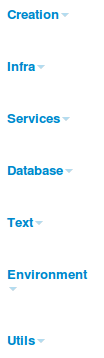
\includegraphics[scale=0.5]{categories.png} 
%%   \end{center}
%%   \caption{Les 7 catégories de commandes qui sont des listes déroulantes} 
%% \end{figure}

Lorsque l'utilisateur clique sur l'une des commandes d'une catégorie, il voit
apparaître en haut de l'application plusieurs champs de saisie qui décrivent les
arguments que doit recevoir la commande.
Il y a un champ de saisi pour un argument.
La commande \textit{restart-services} prend le nom d'une infra en
arguments. Elle possède donc un champ ``infra...''.
La commande \textit{update-env-file} prend le nom d'une infra et le chemin du
fichier de description de mise à jour de l'infra en arguments. Elle possède donc
un champ ``infra...'' et un sélecteur de fichier.

\begin{figure}[H]
  \begin{center}
    
\includegraphics[scale=0.5]{champ-update-env-file.png} 
  \end{center}
  \caption{Commande update-env-file} 
\end{figure}

\subsection{Sélecteur de fichier}

Un sélecteur de fichier est ajouté pour les commandes \textit{create},
\textit{migrate} et \textit{update-env-file} de l'outil d'infra.

Lorsque l'utilisateur clique sur le bouton 'Execute', le fichier sélectionné est
uploadé vers le serveur et la commande elle-même est exécutée coté serveur avec
le fichier qui vient d'être téléchargé.
Du code Ajax est utilisé pour ne pas avoir besoin de recharger la page lors de
l'envoie du fichier.
Ainsi le client peut recevoir l'output de la commande dans la page web.

 \section{Restructuration du code JavaScript}
 
 La quantité de code JavaScript est devenue conséquente. Une restructuration du
 code s'impose pour améliorer sa lisibilité, simplifier sa maintenance et
 faciliter l'ajout de nouvelles fonctionnalités.

\subsection{RequireJS}

Dans un langage de programmation comme Java, on ne se soucie pas du chargement
des dépendances. Il suffit de les définir (import java.utils.Collection par
exemple) et la JVM s'occupe de charger les modules de façon complètement
transparente pour le développeur.

Au contraire de ces langages évolués, la gestion des dépendances n'est pas
une tâche simple en JavaScript.
JavaScript ne possède pas de système de modules intelligent, ce qui rend le
découpage de code difficile.

Prenons un exemple. Les dépendances sont représentées comme des flèches du
module du client à gauche jusqu'au module requis à droite :

module1 $\rightarrow$ module2 $\rightarrow$ module3, module4 

En JavaScript, à chaque fois que module1 est utilisé, tous les autres modules
doivent être importés dans le bon ordre de la façon suivante :

\lstset{language=XML}
\begin{lstlisting}
  <script type="text/javascript" src="module4"></script
  <script type="text/javascript" src="module3"></script>
  <script type="text/javascript" src="module2"></script>
  <script type="text/javascript" src="module1"></script>
\end{lstlisting}

Heureusement, il existe quand même des moyens de définir de telles hiérarchies de
dépendances en JavaScript. RequireJS est une bibliothèque qui rend possible la
définition de dépendances entre modules de manière approprié pour le navigateur.
RequireJS est une sorte de \#include/import/require pour JavaScript.\\
Voici un extrait de code de l'application utilisant RequireJS :
\lstset{language=JavaScript}
\begin{lstlisting}[caption=Définition du module commands avec RequireJS]
  define(
  // La liste des dépendances 
  // en python: import jquery, bootstrap-typeahead, bootstrap-button, bootstrap-dropdown
  ['jquery', 'bootstrap-typeahead', 'bootstrap-button', 'bootstrap-dropdown'], 
  function(dollar) { 
    // RequireJS assure que les quatre dépendances seront chargées et accessibles à
    // l'intérieur de la fonction.
    
    // définition de la fonction commands
    function commands(webSocketURL, listInfrasSocketURL) = {
      ...
    }
    
    // Utilisation du return pour exporter la fonction commands.
    // Tout ce qui n'est pas exporté reste privé au module.
    return commands;
  }
\end{lstlisting}


\subsubsection{Bénéfique pour la qualité du code}

\textit{\underline{Des APIs et namespace plus propres}}\\

La définition de modules avec RequireJS force le développeur à réfléchir à la
façon dont le module va partager les variables. Forcer le développeur à décider
ce qu'il veut exposer et quels sont les détails d'implémentation spécifiques
qui doivent être cachés conduisent à une meilleure encapsulation du code.

En plus, lorsque le développeur importe un module avec RequireJS, les propriétés
et méthodes exportées par le module sont accessibles à travers une variable
``package''. Ça permet à deux modules différents d'exporter un attribut avec le
même nom sans que l'un d'eux ne cache la valeur de l'autre.

\subsubsection{Bénéfique pour les performances}

\textit{\underline{Charger de plus petites ressources avec moins de requêtes}}\\

Deux principaux facteurs affectent le chargement d'une page :
\begin{itemize}
\item La taille des ressources. Le temps de chargement augmente avec la taille
  des ressources.
\item Le nombre de ressources. Plus il y a de ressources plus le nombre de
  requêtes augmente.
\end{itemize}

La meilleur approche pour gérer le premier cas est de ``minifier'' le code.
Minifier consiste à supprimer tous les caractères du code qui sont seulement
utiles pour rendre le code plus lisible (des espaces et retours à la ligne
entre autres).

Pour diminuer le nombre de requêtes HTTP, la solution habituelle (sans rentrer
dans la mise en cache) est de regrouper tous les fichiers dans un seul sans
modifier le code. De cette manière, le nombre de requêtes requises pour
récupérer les ressources du serveur est réduit à une seule.

RequireJS fourni un outil pour automatiquement minifier et
regrouper tous les modules en un seul. Cet outil est capable de minifier chaque
fichier CSS du projet et minifier et regrouper tous les fichiers JavaScript dont
les dépendances ont été définies en tant que module RequireJS.

\subsection{CoffeeScript}

Pour éviter de retomber dans les nombreux pièges rencontrés au cours du
développement de la partie cliente en JavaScript, j'ai décidé d'utiliser
CoffeeScript à la place de JavaScript.

CoffeeScript est un langage influencé par ruby qui fourni, entre autres choses,
les compréhensions de listes, une meilleure gestion des variables sans polluer
le namespace et plein d'autres outils qui rendent le développement JavaScript
plus simple. CoffeeScript compile vers du JavaScript lisible et bien formatté,
ce qui facilite le débugage.
Tout le code JavaScript écrit jusqu'ici est traduit en CoffeeScript.
Le code est plus concis (gain de $\sim$15\% pour le nombre de lignes de code) et le
développement plus fluide.

\section{Messages Done et Failed}

Lorsqu'une commande se termine, l'utilisateur reçoit un message ``Done'' si la
commande a réussi ou un message ``Failed!'' si la commande a échouée.

\begin{figure}[H]
  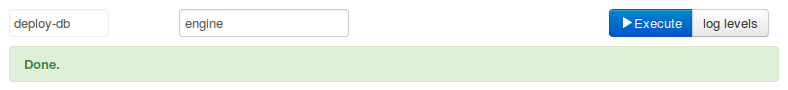
\includegraphics[width=\textwidth]{cmdDone.png}
  \caption{Déploiement réussi de la base de données pour l'infra engine}
\end{figure}

Un message ``Failed!'' est accompagné de l'exception Scala émise par
l'application.

\begin{figure}[H]
  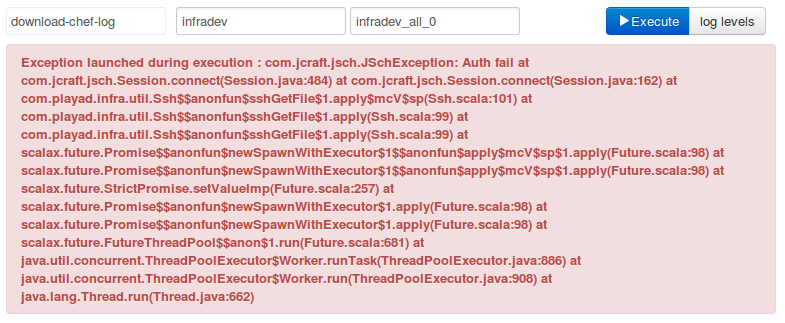
\includegraphics[width=\textwidth]{cmdFailed.png}
  \caption{Échec de la récupération des logs Chef sur le nœud infradev\_all\_0.\\
    L'application ne peut apparemment pas se connecter sur l'instance EC2 de
    ce nœud car l'authentification a échoué}
\end{figure}

\section{Verroux sur les commandes à effet de bord}

\textit{La demande} : interdire l'exécution de deux commandes identiques en même temps si
celles-ci ont des effets de bord.

L'application web coté serveur enregistre les commandes en cours d'exécution.
À chaque nouvelle exécution d'une commande, l'application verrouille toute autre
exécution de la même commande. Lorsque la commande est terminée, qu'elle ait
réussie ou qu'elle ait échouée, l'application enlève le verrou.

Si un utilisateur exécute une commande qui est déjà en cours d'exécution par un
autre utilisateur, l'application renvoie alors un message d'alerte à
l'utilisateur lui indiquant que sa commande est refusée.

\begin{figure}[H]
  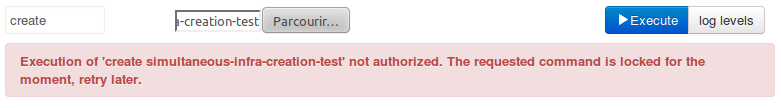
\includegraphics[width=\textwidth]{cmdLocked.png}
  \caption{La commande 'create simultaneous-infra-creation-test' est déjà en
    cours d'exécution.}
\end{figure}

Certaines commandes n'ont pas de verrou car elles n'ont pas d'effet de bord.
Par exemple les commandes status, status-services et show n'ont pas besoin
de verrou car elles ne font que récupérer des informations concernant une infra.

\section{Transformer l'outil d'infra en bibliothèque}

\textit{La demande} : pouvoir appeler les méthodes de l'outil d'infra via l'application
web. Mais, très important, l'outil doit toujours fonctionner en ligne de
commande.

\textit{L'objectif} : transformer l'outil d'infra en bibliothèque.
Le jar de l'outil d'infra pourra ensuite être intégré à l'application web.

La transformation de l'outil d'infra en API impose plusieurs changements.

\subsection{Des singletons transformés en simples classes}

Toutes les classes étaient des services. Elles étaient toutes des singletons.
Les services proposent des méthodes utilitaires et n'ont pas d'état. Il était
donc logique d'avoir des singletons car nous n'avions pas besoin de plus d'une
instance par service. 

De même, il existait un singleton Logger qui était utilisé par tous les autres
singletons afin de logguer leurs différentes actions.

Dans l'outil d'infra en ligne de commande, un seul logger suffisait, un simple
logger qui enregistre tout dans un fichier.
Mais pour que l'outil se transforme en API, l'utilisateur doit avoir le
controle sur le logger. L'utilisateur doit pouvoir choisir son logger, il doit
pouvoir en utiliser plusieurs si il souhaite.

C'était en effet le cas de l'application web qui allait être le premier
programme à utiliser l'API. L'application web a besoin de plusieurs
loggers. Elle a en fait besoin d'un logger par internaute.
Une nouvelle instance du Logger est créée pour chaque nouvel internaute afin
que les résultats des commandes lancées par un internaute soient isolés dans son
propre fichier. Les logs des internautes ne doivent pas être mélangés.

Un refactoring important a permis la transformation de l'outil d'infra en API.
Tous les singletons sont transformés en simples classes.
Puisqu'il n'existe plus de singleton, les constructeurs de ces classes prennent
alors en paramètre les instances d'autres classes dont elles dépendent.

Par chance, l'outil d'infra a été développé avec un langage statiquement
typé, Scala en l'occurence.
Lorsqu'un singleton se transforme en simple classe, le code extérieur qui
utilisait ce singleton doit changer sa façon de l'appeler.

Grace au typage statique, Eclipse affichait les erreurs de compilation dans
les différents fichiers faisant usage de la classe modifiée. Il suffisait alors
de suivre ces erreurs et de les corriger.

\subsection{Libération mémoire du cache}

L'outil faisait aussi utilisation d'un cache pour l'optimisation de méthodes
appelées plusieurs fois durant l'exécution d'une même commande.

Puisque ce programme était conçu pour exécuter une seule commande, la
consommation mémoire de ce cache ne posait pas problème.
À la fin de l'exécution de la commande, le programme se termine et la JVM
se charge de libérer la mémoire allouée.

Dans le cadre d'une API, le problème est différent. Le client qui utilise l'API
de l'outil d'infra ne souhaite peut-être pas exécuter une seule commande.
Si le client exécute plusieurs commandes succésives, le cache grossit pour
chaque nouvelle commande exécutée et consomme de plus en plus de mémoire.

C'est le cas de l'application web dont la durée d'exécution est \textit{supposée}
infinie. Une fois mise en production, l'application web doit être
continuellement disponible pour les utilisateurs. Seul le déploiement d'une
nouvelle version de l'application web doit engendrer son redémarrage.

Pour corriger ce problème, les données relatives à une commande sont supprimées
du cache lorsque l'exécution de cette commande se termine.

\subsection{Des types de retour significatifs}

Plusieurs méthodes ne renvoyaient rien. Certaines d'entre elles ont été
modifiées pour qu'elles aient un type de retour plus riche.

Par exemple, la commande 'list' affiche sur la sortie standard la liste de
toutes les infrastructures existantes.
Son type de retour était Unit (void en Java) et devient Seq[Infra] (en Java, le
type le plus proche serait List<Infra>).
Le client de l'API peut alors se servir de la liste des infrastructures retournée.

\section{Fonctionalités de la webapp}

\subsection{Complétion automatique des infras}

L'application web fournie une complétion automatique des noms d'infrastructures
pour les champs qui requièrent une infra.

\begin{figure}[H]
  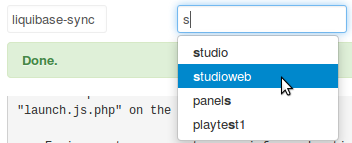
\includegraphics[scale=1]{auto-completion.png}
  \caption{Complétion automatique des noms d'infrastructures disponibles}
\end{figure}

La liste déroulante assiste l'utilisateur lorsqu'il doit indiquer
l'infrastructure sur laquelle s'appliquera sa commande.
Cette fonctionnalité améliore l'expérience utilisateur, l'utilisateur gagne du
temps et évite les erreurs de frappe.

C'est le plugin JavaScript Typeahead de Twitter Bootstrap qui est utilisé pour
avoir ce design sympathique. L'internaute tape quelques lettres de l'item qu'il
recherche et le plugin affiche les items qui contiennent cette séquence de
lettres en facteur.

Une fois le plugin inclus dans le projet, il faut renseigner l'attribut
\textit{data-source} de la balise input avec les différents choix possibles de
la liste.

\lstset{language=XML}
\begin{lstlisting}[caption=utilisation de bootstrap-typeahead]
  <input type="text" data-provide="typeahead" data-items="4" data-source='[]'>
\end{lstlisting}

Comme présenté dans le code html ci-dessus, la liste est vide au début.
Elle contiendra la liste des infras disponibles qui sera générée coté serveur.

Lorsque l'utilisateur se connecte à l'application, la page web lui est envoyée
instantanément. Il peut exécuter la commande qu'il souhaite mais ne
dispose pas encore de la complétion automatique des infrastructures.

Une WebSocket est utilisée pour remplir dynamiquement cette liste.
En asynchrone, la commande \textit{list} est exécutée coté serveur.
Cette commande récupère la liste de toutes les infrastructures disponibles en
requêtant Chef qui dispose de cette information. La commande \textit{list} met
environ 5 secondes à s'exécuter sur l'instance EC2 qui héberge l'application
web.
Une fois la commande \textit{list} terminée, le serveur envoie cette liste des
infrastructures au client via la WebSocket.
Une fonction JavaScript renseigne alors l'attribut data-source avec
la liste des infrastructures reçue.

Le client ne ressent aucune latence de l'application car les briques essentielles
de l'interface web pour exécuter une commande sont instantanément disponibles.
Les fonctionnalités complémentaires comme l'auto-complétion viennent se greffer
dynamiquement à l'interface et n'altèrent pas la navigation de l'utilisateur.


\subsection{Défilement automatique des logs de la commande en cours d'exécution}

\begin{figure}[H]
  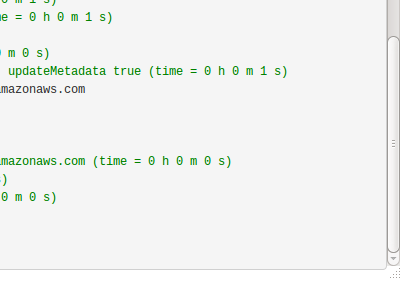
\includegraphics[width=0.50\textwidth]{defilement-automatique-1.png}
  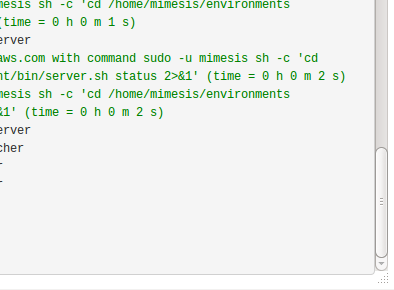
\includegraphics[width=0.50\textwidth]{defilement-automatique-2.png}
  \caption{Défilement automatique des logs - exécution de la commande
    status-services panel\\L'image de droite est prise 4 secondes après celle de gauche}
\end{figure}

Lorsqu'une nouvelle ligne est ajoutée à la suite de l'output du résultat de la
commande, la barre de défilement se met automatiquement en bas.

Si l'utilisateur déplace la barre de défilement, le défilement automatique se
désactive.
Si l'utilisateur replace manuellement la barre de défilement tout en bas,
le défilement automatique est de nouveau actif.

%% \subsection{couleurs des logs}
\subsection{Contrôler les niveaux de log}

Avant d'exécuter une commande, les niveaux de logs peuvent être activés ou
désactivés. Les informations affichées au cours de l'exécution de la commande
sont alors filtrées pour n'afficher que celles correspondant aux niveaux de logs.
Il y a cinq niveaux de logs utilisés dans l'application : 
Trace, Debug, Info, Warn et Error.
Par défaut, tous les niveaux de logs sont activés.

\begin{figure}[H]
  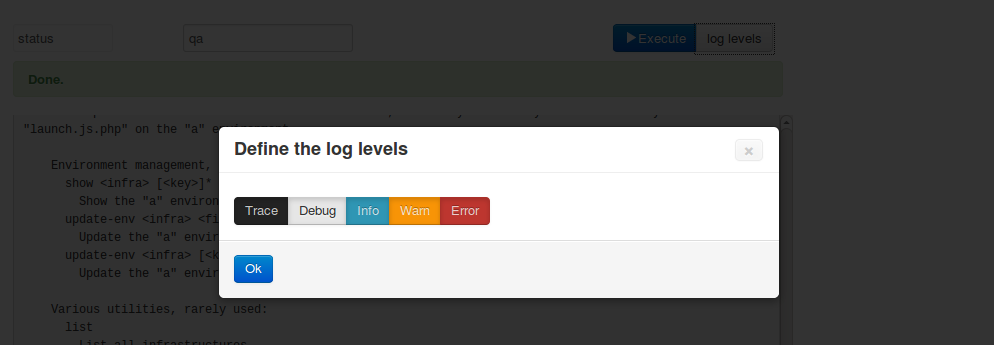
\includegraphics[width=\textwidth]{log-levels.png}
  \caption{Tous les niveaux de logs sont activés}
\end{figure}

\bigskip

La commande \textit{status} fait un appel au logger.debug durant son exécution.
Un utilisateur laissera le niveau Info actif et désactivera Debug
si il souhaite uniquement recevoir le résultat du \textit{status} et ne veut pas
être encombré des tous les logs de Debug.
Du coup, lors de l'exécution de la commande \textit{status qaz}, la ligne
\verb?EXEC: Perform get on data/infrastructures/qaz? ne sera pas affichée car le
niveau Debug a été désactivé par l'utilisateur.



\subsection{La commande download-chef-log}
La création et la mise à jour d'une infra sont des tâches délicates qui peuvent
souvent échouer.
La cause de cet échec peut varier.
Ça peut venir par exemple de la création de la base de donnée RDS qui ne s'est
pas correctement terminée comme ça peut aussi venir de la limite du nombre de
groupes de sécurité fixée par Amazon qui est atteinte.

Mais la cause la plus fréquente est l'échec de l'exécution du chef-client.
À chaque fois que ce programme plante, un adminastreur système récupère le
fichier de logs Chef pour connaître la cause. Il recherche sur amazon l'url de
l'instance EC2 qui héberge l'infrastructure car c'est cette instance qui exécute
chef-client et qui possède les logs Chef. Une fois cette url trouvée, il peut se
connecter à l'instance via ssh et récupérer le fichier de log.

Pour éviter cette tâche fastidieuse aux administrateurs systèmes, la commande
\textit{download-chef-log} a fait son apparition dans l'application web.

Depuis l'interface web, il suffit de renseigner deux champs pour récupérer le
fichier de log. Un premier champ contient le nom de l'infrastructure et un
deuxième contient le nom du nœud sur lequel la commande a échoué.

Contrairement à l'url de l'instance qui n'était pas connu par l'administrateur
système et qu'il devait rechercher sur Amazon, il connaît déjà le nom d'infra et
le nom du nœud.

De plus, pour faciliter son utilisation, les deux champs de cette nouvelle
commande \textit{download-chef-log} possèdent la complétion automatique.

\begin{figure}[H]
  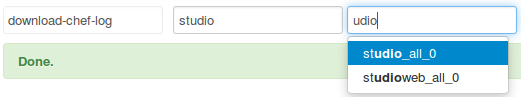
\includegraphics[width=\textwidth]{completion-download-chef-log.png}
  \caption{Complétion automatique disponible aussi pour la liste des nœuds}
\end{figure}

À partir du nom de l'infra et du nœud, le serveur web requête Chef pour
connaître l'url de l'instance EC2 correspondante. En utilisant la commande
\textit{scp}, le serveur copie le fichier de logs Chef distant dans un
dossier local publique.
L'application génère ensuite une URL qui pointe sur le fichier local téléchargé
et envoie cette URL au client.
L'URL est alors affichée sur la page web de l'utilisateur. Il lui suffit de
cliquer dessus pour télécharger le fichier de log qu'il recherchait.


\begin{figure}[H]
  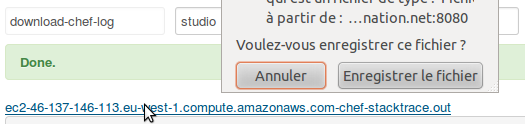
\includegraphics[width=\textwidth]{download-chef-log.png}
  \caption{Lien de téléchargement du fichier de log généré par la commande \textit{download-chef-log}}
\end{figure}

\section{Évolutions de l'outil d'infra}
TODO
\subsection{création d'infrastructure}
\subsection{optimisations en temps d'exécution}
\subsection{documentation dans le wiki}

%% - afficher les logs du chef-client dans la sortie web lors d'une création
%% d'infra.

%% - J'ai écris le code qui créé un nouveau db security group rds à chaque fois
%% qu'une nouvelle infra est créée.
%% Ça permetra d'éviter la limite qu'on atteint rapidement lorsqu'on utilise le
%% security group 'default'.

%% - J'ai rajouté un check dans l'outil d'infra pour interdire le create sur une
%% t1.micro parce-que la création d'infra sur une t1.micro ne fonctionne pas, pas
%% assez de mémoire disponible sur les micros probablement.
%% J'ai rajouté un autre check qui vérifie que le nom de l'infra ne contient pas de
%% majuscule.

%% - Documentation dans le wiki de ce que fait un create infra, un destroy infra.
%% J'ai listé toutes les étapes.

%% - optimisation en temps d'exécution de quelques commandes de l'outil d'infra.
%% registerAllDns est maintenant exécuté en parallèle, chaque
%% registerDNS est indépendant et peut être exécuté dans son propre thread.

%% - réduit de 10 secondes le CreateInfra. La liste des instances rds était requêtée
%% deux fois sans aucun changement entre les deux listes. J'ai juste supprimé une
%% requête et stocké la liste dans une variable.
%% (dans initRds, val rdsList = rds.list)

%% - Faire en sorte de pouvoir créer des infras même sans service mongodb.

%% - rajout des couleurs pour les lignes de l'output.
%% Lorsque la ligne commence par :
%% FAIL -> colore en rouge
%% WARN -> colore en jaune
%% DONE -> colore en vert
%% Lorsque la ligne contient le mot Exception -> colore en rouge

\section{Plugin SBT}
TODO

%% - packaging SBT
%% - création d'un plugin qui standardise le déploiement d'une application web.
%% (exemple du déploiement automatisé d'une application Play! :
%% récupérer l'archive depuis un bucket S3 ;
%% le dézipper ;
%% va chercher dans le databag Chef le fichier de configuration à appliquer
%% lorsqu'on souhaite déployer une application Play (ie le fichier
%% application.conf) ;
%% avec le template du fichier application.conf du databag, rempli les champs
%% manquants du fichier configurations/application.conf de l'archive dézippé ;
%% exécute le script scripts/start.sh





